%% optional
\appendixtitles{no} %Leave argument "no" if all appendix headings stay EMPTY (then no dot is printed after "Appendix A"). If the appendix sections contain a heading then change the argument to "yes".
\appendixsections{multiple} %Leave argument "multiple" if there are multiple sections. Then a counter is printed ("Appendix A"). If there is only one appendix section then change the argument to "one" and no counter is printed ("Appendix").

\newpage

\appendix
\section{}
\subsection{Tables}

\begin{table}[h]
\begin{adjustwidth}{-4cm}{}
\caption{Measured pyrethroids metabolites and the limits of detection across each NHANES cycle.}
\label{tab:tabs1}
\begin{tabular}{lrrrrrrr}
\toprule
  & 1999-2000 & 2001-2002 & 2007-2008 & 2009-2010 & 2011-2012 & 2013-2014 & 2015-2016\\
\midrule
3PBA & 0.1 & 0.1 & 0.1 & 0.1 & 0.1 & 0.1 & 0.1\\
FPBA & 0.2 & 0.2 & 0.1 & 0.1 & 0.1 & 0.1 & 0.1\\
trans-DCCA & 0.4 & 0.4 & 0.6 & 0.6 & 0.6 & 0.6 & 0.6\\
DBCA & 0.1 & 0.1 & 0.5 & 0.5 &  &  & \\
cis-DCCA & 0.1 & 0.1 &  &  &  &  & \\
\bottomrule
\end{tabular}
\end{adjustwidth}
\end{table}


\begin{table}[H]
\begin{adjustwidth}{-4cm}{}
\caption{\label{tab:tabs2}Pyrethroid parent compounds and corresponding metabolites.}
\begin{tabular}[t]{lccccc}
\toprule
  & 3PBA & FPBA & DBCA & cis-DCCA & trans-DCCA\\
\midrule
Cyfluthrin &  & x &  & x & x\\
Cypermetrhin & x &  &  & x & x\\
Deltamethrin & x &  & x &  & \\
Permethrin & x &  &  & x & x\\
\bottomrule
\end{tabular}
\end{adjustwidth}
\end{table}


\begin{table}[h]
\begin{adjustwidth}{-4cm}{}
\caption{Summary of key PBK parameters related to urine pyrethroid metabolites.}
\label{tab:tabs3}
\centering
\small
\begin{tabular}{lllrr}
\toprule
Parameter & Description & Unit & Value & Reference\\
\midrule
BW & Body Weight & kg & Observed & \\
UrineCreatinine & Urine Creatinine & mg creatinine / dl urine & Observed & \\
DailyCreatinine & Daily Creatinine & mg creatinine / day & Estimated & \cite{stanfield2022bayesian}\\
DLM\_KA & Uptake rate of deltamethrin & /h & 1.51 & \cite{quindroit2019estimating}\\
cisPRM\_KA & Uptake rate of cis-permetrhin & /h & 0.52 & \cite{quindroit2019estimating}\\
tranPRM\_KA & Uptake rate of trans-permethrin & /h & 1.3 & \cite{quindroit2019estimating}\\
cisCPM\_KA & Uptake rate of cis-cypermethrin & /h & 0.52 & \cite{quindroit2019estimating}\\
tranCPM\_KA & Uptake rate of trans-cypermethrin & /h & 1.3 & \cite{quindroit2019estimating}\\
cisCYF\_KA & Uptake rate of cis-cyfluthrin & /h & 0.52 & \cite{quindroit2019estimating}\\
tranCYF\_KA & Uptake rate of trans-cyfluthrin & /h & 1.3 & \cite{quindroit2019estimating}\\
DLM\_Kfec & Fecal excretion rate of deltamethrin & /h & 0.59 & \cite{quindroit2019estimating}\\
cisPRM\_Kfec & Fecal excretion  rate of cis-permetrhin & /h & 0.39 & \cite{quindroit2019estimating}\\
tranPRM\_Kfec & Fecal excretion  rate of trans-permethrin & /h & 0.85 & \cite{quindroit2019estimating}\\
cisCPM\_Kfec & Fecal excretion rate of cis-cypermethrin & /h & 0.39 & \cite{quindroit2019estimating}\\
tranCPM\_Kfec & Fecal excretion rate of trans-cypermethrin & /h & 0.85 & \cite{quindroit2019estimating}\\
cisCYF\_Kfec & Fecal excretion  rate of cis-cyfluthrin & /h & 0.39 & \cite{quindroit2019estimating}\\
tranCYF\_Kfec & Fecal excretion  rate of trans-cyfluthrin & /h & 0.85 & \cite{quindroit2019estimating}\\
DLM\_3PBA & Metabolic fraction of deltamethrin to 3PBA & - & 0.15 & \cite{quindroit2019estimating}\\
DLM\_DBCA & Metabolic fraction of deltamethrin to DCCA & - & 0.73 & \cite{quindroit2019estimating}\\
cisPRM\_3PBA & Metabolic fraction of cis-permethrin to 3PBA & - & 0.37 & \cite{quindroit2019estimating}\\
cisPRM\_DCCA & Metabolic fraction of cis-permethrin to DCCA & - & 0.37 & \cite{quindroit2019estimating}\\
transPRM\_3PBA & Metabolic fraction of trans-permethrin to 3PBA & - & 0.85 & \cite{quindroit2019estimating}\\
transPRM\_DCCA & Metabolic fraction of trans-permethrin to DCCA & - & 0.61 & \cite{quindroit2019estimating}\\
cisCPM\_3PBA & Metabolic fraction of cis-cypermethrin to 3PBA & - & 0.16 & \cite{quindroit2019estimating}\\
cisCPM\_DCCA & Metabolic fraction of cis-cypermethrin to DCCA & - & 0.32 & \cite{quindroit2019estimating}\\
transCPM\_3PBA & Metabolic fraction of trans-cypermethrin to 3PBA & - & 0.39 & \cite{quindroit2019estimating}\\
transCPM\_DCCA & Metabolic fraction of trans-cypermethrin to DCCA & - & 0.57 & \cite{quindroit2019estimating}\\
cisCYF\_FPBA & Metabolic fraction of cis-cyfluthrin to FPBA & - & 0.1 & \cite{quindroit2019estimating}\\
cisCYF\_DCCA & Metabolic fraction of cis-cyfluthrin to DCCA & - & 0.27 & \cite{quindroit2019estimating}\\
transCYF\_FPBA & Metabolic fraction of trans-cyfluthrin to 3PBA & - & 0.23 & \cite{quindroit2019estimating}\\
transCYF\_DCCA & Metabolic fraction of trans-cyfluthrin to DCCA & - & 0.35 & \cite{quindroit2019estimating}\\
\bottomrule
\end{tabular}
\end{adjustwidth}
\end{table}


\begin{table}
\begin{adjustwidth}{-4cm}{}
\caption{\label{tab:tabs4}Distribution of PBK parameters used in Monte Carlo simulation for exposure risk assessment.}
\begin{tabular}[t]{lccc}
\toprule
Parameter type & No. of parameter & SD & Truncation (±nxSD)\\
\midrule
Plasma unbound fraction & 1 & 0.1 & 2\\
Partition coefficient & 7 & 0.3 & 3\\
Permeability area cross product & 3 & 0.3 & 3\\
Uptake and fecal excretion rate & 2 & 0.4 & 3\\
Clearance rate & 2 & 0.4 & 3\\
\bottomrule
\end{tabular}
\end{adjustwidth}
\end{table}


\begin{table}[h]
\begin{adjustwidth}{-4cm}{}
\caption{Summary of detection rate (\%) for each prethroid metabolites across each NHANES cycle.}
\label{tab:tabs6}
\begin{tabular}{llcccccl}
\toprule
 & 1999-2000 & 2001-2002 & 2007-2008 & 2009-2010 & 2011-2012 & 2013-2014 & 2015-2016\\
\midrule
3PBA & 68.74 & 77.04 & 65.02 & 72.34 & 91.00 & 88.25 & 95.70\\
FPBA & 3.04 & 0.49 & 6.55 & 4.63 & 15.34 & 10.18 & 13.02\\
trans-DCCA & 33.24 & 28.31 & 15.83 & 11.62 & 7.65 & 24.62 & 37.49\\
DBCA & 0.63 & 0.88 & 1.46 & 1.48 &  &  & \\
cis-DCCA & 41.59 & 33.08 &  &  &  &  & \\
\bottomrule
\end{tabular}
\end{adjustwidth}
\end{table}

\subsection{Figures}

\begin{figure}[h]
\begin{adjustwidth}{-4cm}{}
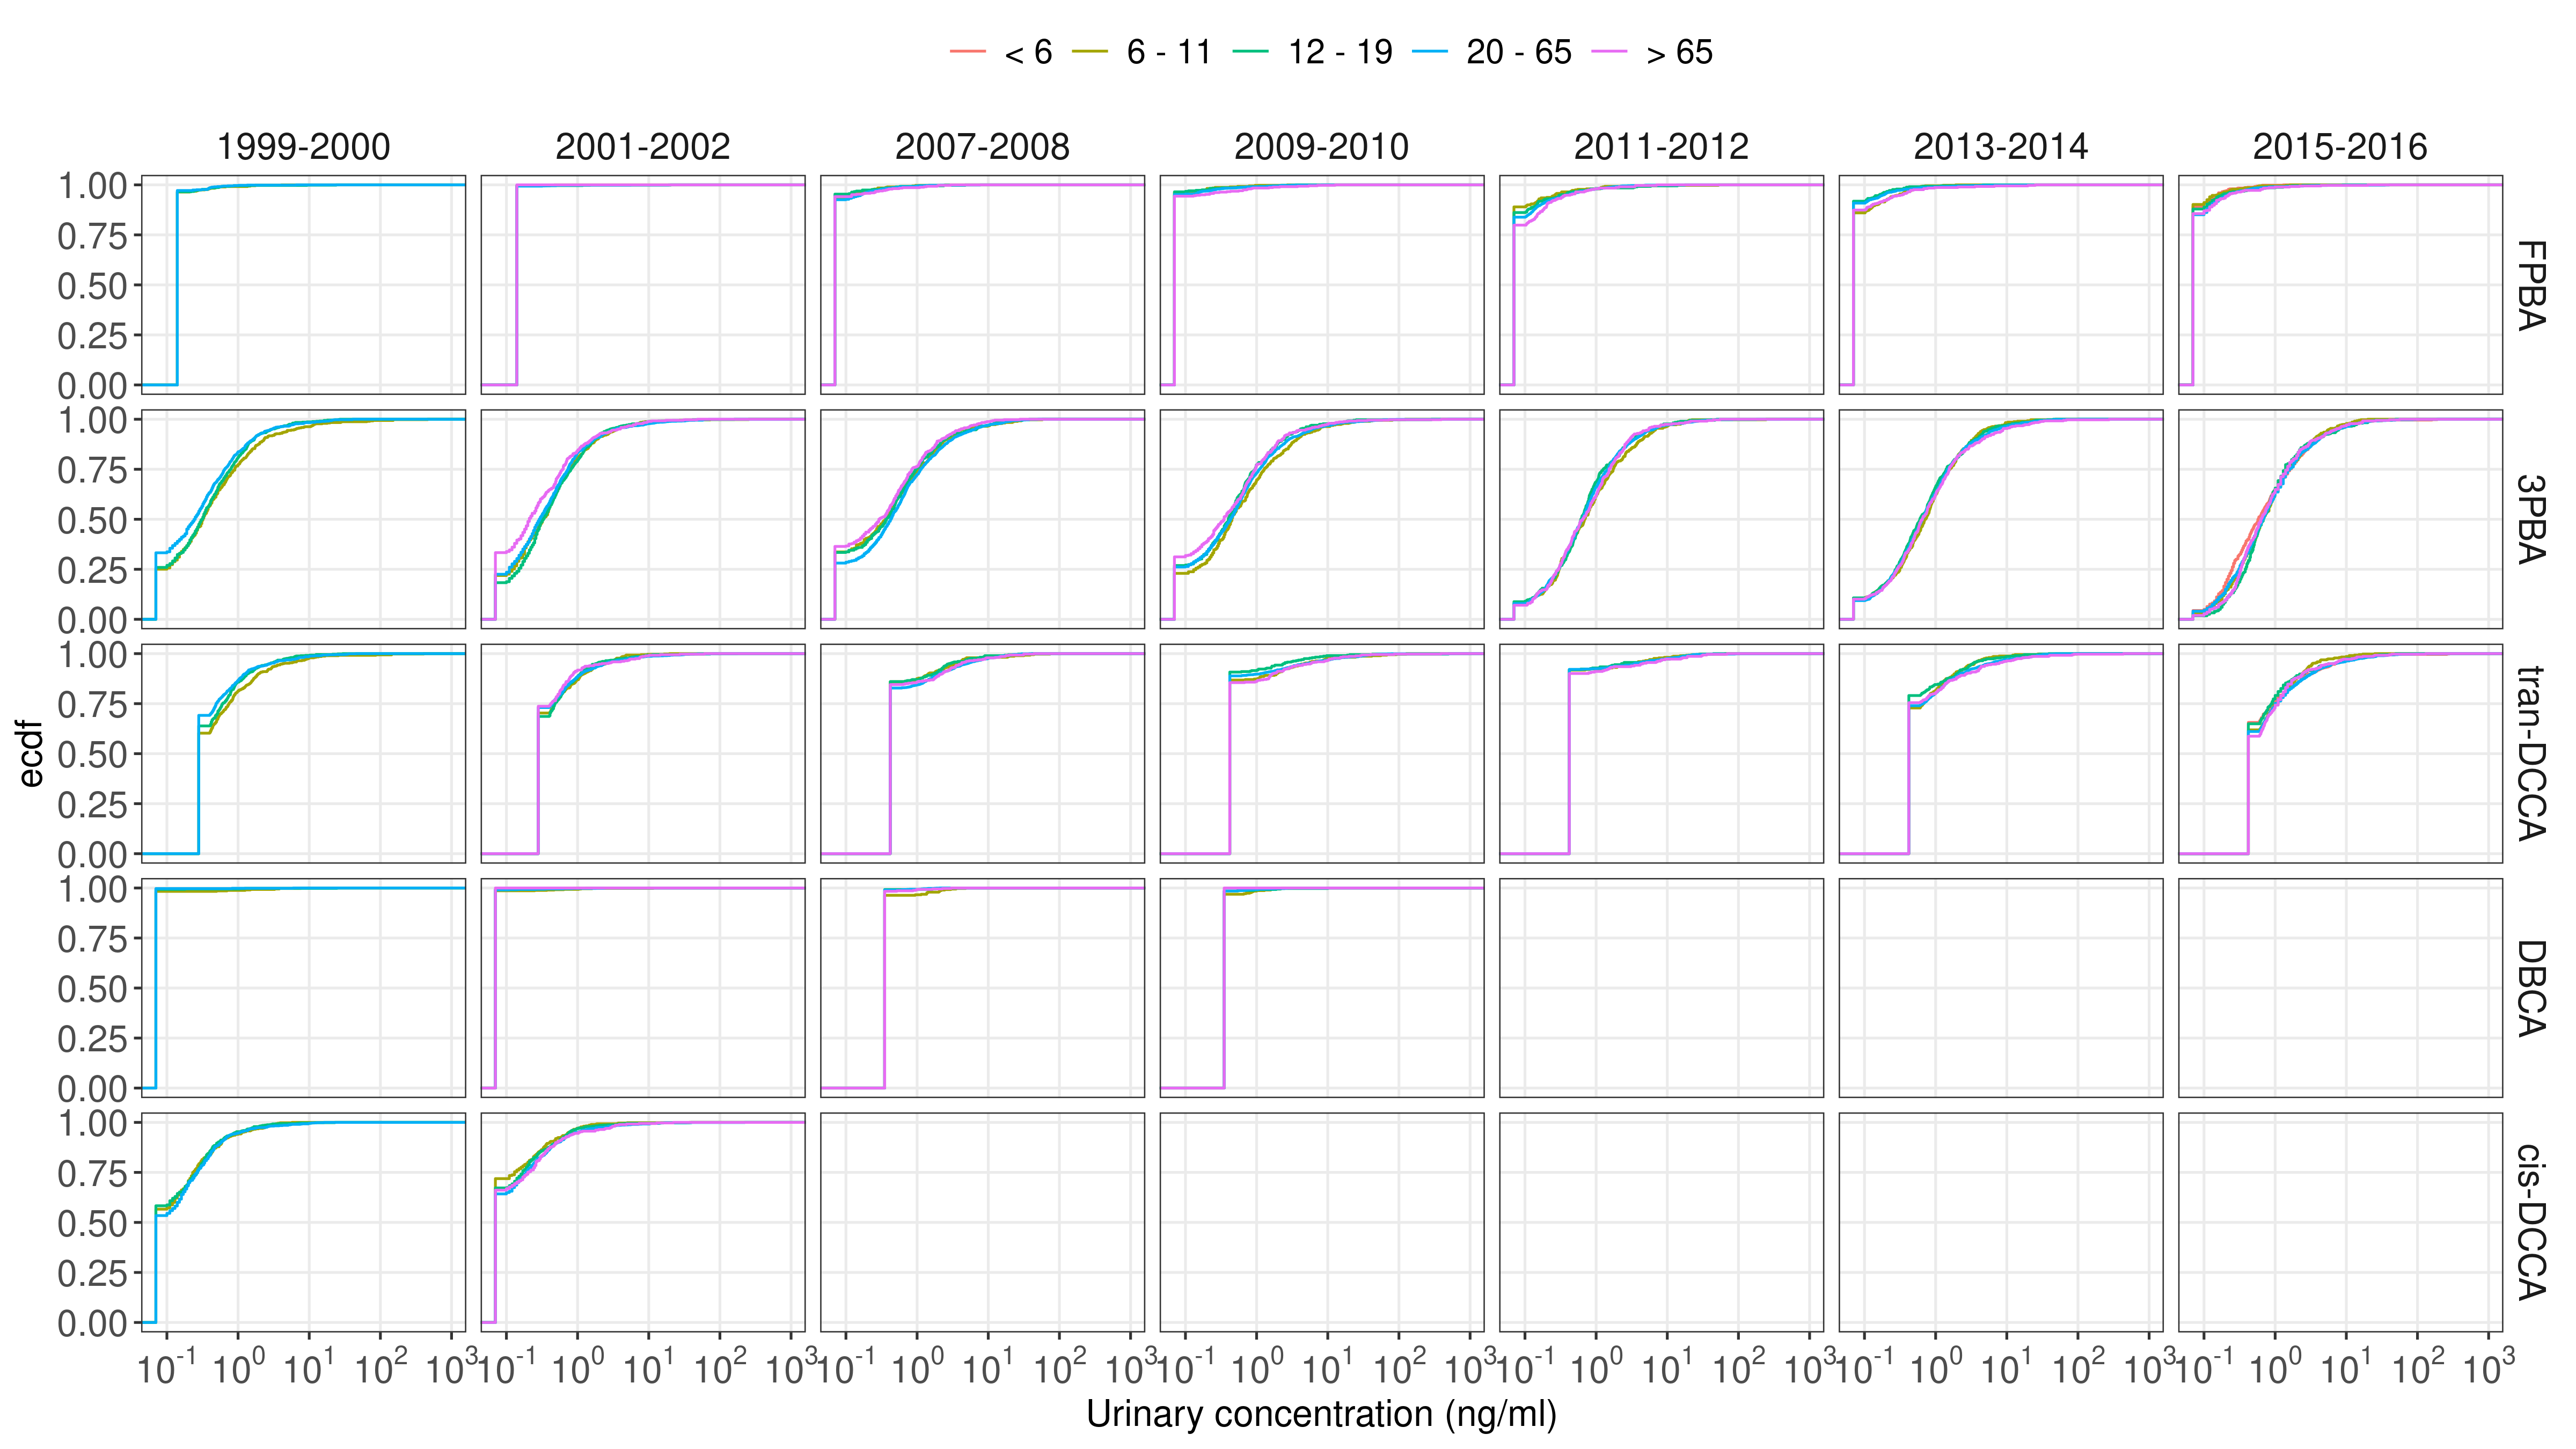
\includegraphics[width=\linewidth]{figures/fig3} 
\hfill
\end{adjustwidth}
\caption{Cumulative distribution of urinary pyrethroid metabolite concentrations across different age groups.}\label{fig:ecdf}
\end{figure}
